%% Standalone Supplementary Information for the NCS submission (separate file, so references to
%% main-text figures/tables are plain numbers): see build.sh; si_clean.tex is the wrapper used by ./build.sh clean.
\documentclass[pdflatex,sn-nature]{sn-jnl}% single-column Supplementary Information


%%%% Standard packages. The sn-jnl class assumes xcolor / textcomp / manyfoot
%%%% are loaded (it uses them in its \begin{document} hook).
\usepackage{graphicx}%
\usepackage{amsmath,amssymb,amsfonts}%
\usepackage{mathtools}%
\usepackage{xcolor}%
\usepackage{textcomp}%
\usepackage{manyfoot}%
\usepackage{booktabs}%
\usepackage{array}%
\usepackage{microtype}%
\usepackage[title]{appendix}%

%% Tighten Springer Nature's default page margins (the class leaves a very
%% large bottom margin and ~24mm sides). This widens the two-column text block
%% and reduces whitespace while keeping the two-column journal layout.
\geometry{a4paper, top=16mm, bottom=18mm, left=18mm, right=18mm,
          marginparwidth=0mm, marginparsep=0mm, bindingoffset=0mm, columnsep=8mm}

\raggedbottom

%% Corresponding-author asterisk. sn-jnl.cls emits it inside
%%   \authorsep{#2}\unskip\ifx\@authfrstarg\empty\else ... {*} ... \fi
%% in \@@corrauthor, where \@authfrstarg is the OPTIONAL affiliation argument.
%% All four authors share one affiliation, so no affiliation superscripts are
%% wanted and \author* is written without brackets -- which skips that branch
%% entirely and leaves the "*Corresponding author(s)" footnote with no asterisk
%% anchored to any name. Redefine the macro to print the asterisk
%% unconditionally, and no affiliation number. (Delete this patch and restore
%% \author*[n] / \affil[n] if a second affiliation is ever added.)
\makeatletter
\renewcommand{\@@corrauthor}[2][]{\def\@authfrstarg{#1}\@corauemailtrue%
  \advance\corraucount by 1%
  \g@addto@macro\artauthors{%
    \global\@auemailtrue%
    \Authorfont%
    \def\baselinestretch{1}%
    \authorsep{#2}\unskip\textsuperscript{*}\unskip%
    \def\authorsep{\au@and~}%
    \global\let\sep\@empty\global\let\@corref\@empty%
  }}%
\makeatother

\begin{document}

\title[Supplementary Information]{Supplementary Information for ``Transfer-Learning
Surrogates for Scalable Multi-Fidelity Bayesian Optimization in Molecular and
Materials Discovery''}

\author{\fnm{Jaewook} \sur{Lee}}

\author{\fnm{Ethan} \sur{Errington}}

\author{\fnm{Christian D.} \sur{Lorenz}}

\author*{\fnm{Miao} \sur{Guo}}\email{miao.guo@kcl.ac.uk}

\affil{\orgdiv{Department of Engineering}, \orgname{King's College London},
\orgaddress{\city{London}, \postcode{WC2R 2LS}, \country{United Kingdom}}}

\abstract{This file contains Supplementary Notes 1--8, Supplementary Figures 1--4 and Supplementary Tables 1--11, which are referred to from the main text. Figure and table
numbers without the ``Supplementary'' prefix refer to the main text.}

\maketitle

%% Supplementary Information content, shared by
%%   si.tex   -> standalone SI file for submission (own title page and reference list;
%%               main-text figures, tables and Methods are cited by plain numbers), and
%%   main.tex -> combined working PDF when built with \def\withSI{1} (see build.sh).

\ifdefined\withSI\section*{Supplementary Information}\fi
%% Supplementary Notes are unnumbered \section*s, so numbered subsections would print as 0.1, 0.2, ...
\setcounter{secnumdepth}{0}

% Supplementary Note counter for Nature/NCS-style references.
% This lets \ref{suppnote:...} print the Supplementary Note number.
\newcounter{suppnotecounter}
\newcommand{\suppnote}[2]{%
  \refstepcounter{suppnotecounter}%
  \section*{Supplementary Note \thesuppnotecounter. #1}%
  \label{#2}%
}

% Supplementary figure/table numbering.
% These make captions appear as "Supplementary Figure 1" and
% "Supplementary Table 1" in standard LaTeX classes.
\setcounter{figure}{0}
\setcounter{table}{0}
\renewcommand{\figurename}{Supplementary Figure}
\renewcommand{\tablename}{Supplementary Table}

\suppnote{Surrogate configurations}{suppnote:mfgp}

Supplementary Table~\ref{supptab:surrogate_config} documents the configuration of each of the eight surrogates. It lists fitting procedures, training lengths, learning rates, weight decay, scaling, predictive representations, kernels and likelihoods or heads, inducing points and floating-point precision. The settings shared by all eight surrogates (candidate pool and standardized features, budget, cost ratio, fidelity schedule, farthest-point initial design, retraining from scratch at every refit, and seeds) are those of Methods~4.2 and~4.10, and the transfer-learning (TL) backbone and head are those of Methods~4.3, with the TL details that the table does not state given in the last subsection of this Note. The three Gaussian processes (GPs) use off-the-shelf configurations from BoTorch 0.10.0 and GPyTorch 1.11, whose fitting procedures, training lengths, scaling and precision differ both from TL and from one another, as documented in the table.

\subsection{GP-base}

GP-base is the autoregressive multi-fidelity GP (MFGP)~\citep{kennedy2000predicting}, implemented as BoTorch 0.10.0's \texttt{SingleTaskMultiFidelityGP}~\citep{balandat2020botorch}. It uses a Mat\'{e}rn-5/2 kernel with automatic relevance determination (ARD) over input dimensions and a linear truncated kernel over fidelity. We used the library's default priors. The unbiased and biased Mat\'{e}rn lengthscales have Gamma(3, 6) and Gamma(6, 2) priors, respectively. The fidelity power has a Gamma(3, 3) prior, and the output scale has Gamma(2, 0.15). The noise variance has a Gamma(1.1, 0.05) prior and a lower bound of $10^{-4}$. The mean is a learned constant. Inputs enter as supplied, with fidelity appended as a 0/1 column and no input transform. Targets from both fidelities are standardized together through the \texttt{Standardize} outcome transform.


\begin{table}[p]
\caption{Configuration of the eight surrogates. Shared settings are given in the text of this Note. `Pooled' denotes a \texttt{StandardScaler} fitted at each refit to sampled low-fidelity (LF) and high-fidelity (HF) inputs or targets together. Input dimension is $d$, and $N$ counts sampled points from both fidelities. The losses $\mathcal{L}_{\mathrm{LF}}$ and $\mathcal{L}_{\mathrm{HF}}$ are mean squared errors on standardized targets. The LF network's output and second-hidden-layer representation are $g^{(L)}$ and $\varphi^{(L)}$, respectively.}
\label{supptab:surrogate_config}
{\fontsize{6.6bp}{7.4bp}\selectfont\setlength{\tabcolsep}{1.5pt}%
\begin{tabular}{@{}>{\raggedright\arraybackslash}p{1.45cm}>{\raggedright\arraybackslash}p{2.75cm}>{\raggedright\arraybackslash}p{1.15cm}>{\raggedright\arraybackslash}p{1.4cm}>{\raggedright\arraybackslash}p{0.85cm}>{\raggedright\arraybackslash}p{1.35cm}>{\raggedright\arraybackslash}p{1.9cm}>{\raggedright\arraybackslash}p{2.55cm}>{\raggedright\arraybackslash}p{1.45cm}@{}}
\toprule
Surrogate & Fitting procedure & Training length & Learning rate & Weight decay & Scaling (inputs; targets) & Representation entering the predictive model & Predictive model (kernel and likelihood, or head) & Inducing points; precision \\
\midrule
\multicolumn{9}{@{}l}{\emph{Gaussian-process (GP) family}} \\
GP-base & BoTorch \texttt{Single\-Task\-Multi\-Fidelity\-GP}; exact marginal likelihood with the library priors$^{a}$, L-BFGS-B & to convergence & -- & none & none; \texttt{Standard\-ize} on the pooled LF and HF targets & the $d$ inputs and a 0/1 fidelity column & Mat\'{e}rn-5/2 ARD in a linear truncated fidelity kernel; constant mean; Gaussian likelihood (noise $\ge 10^{-4}$); s.d. of the latent function & none (exact); float64 \\
GP-DKL & GPyTorch \texttt{ExactGP}; exact marginal likelihood, Adam & 500 steps & $10^{-3}$ network; $10^{-2}$ GP parameters & none & none; none & network $d \to 64 \to 64 \to 16$ ($\tanh$), rescaled to $[-1, 1]$; fidelity as task index & radial basis function (RBF) ARD over the 16 features $\times$ index kernel (2 levels, rank 1); constant mean; Gaussian likelihood; no priors; s.d. includes the noise & none (exact); float32 \\
GP-SV & GPyTorch \texttt{ApproximateGP}; variational evidence lower bound (ELBO) over the full training set, Adam & 500 steps & $10^{-2}$ & none & none; none & the $d$ inputs; fidelity as task index & RBF ARD $\times$ index kernel (2 levels, rank 1); constant mean; Gaussian likelihood; Cholesky variational distribution; no priors; s.d. includes the noise & $\min(100,$ $N)$; a random subset of the training inputs, learned; float32 \\
\midrule
\multicolumn{9}{@{}p{15.54cm}}{\emph{Transfer-learning (TL) family: the base surrogate TL-base and the variants TL-PtJ (pretrain-then-joint), TL-E2E (end-to-end joint), TL-SPS (soft parameter sharing) and TL-MMD (domain adaptation, maximum-mean-discrepancy penalty, MMD).} All five: backbone LF network $d \to 64 \to 64 \to 1$ ($\tanh$) and a residual network $[x, g^{(L)}(x)] \to 64 \to 64 \to 1$ of the same form, trained in every configuration as an auxiliary loss branch; full-batch Adam on the mean squared error; HF prediction from the Bayesian linear-regression (BLR) head on $[\,g^{(L)}, \varphi^{(L)}, 1\,]$ (Supplementary Note~\ref{suppnote:blr}), LF predictive distribution for calibration from the LF BLR head with $\alpha = \beta = 1$; no inducing points; networks in float32, BLR heads in float64.} \\
TL-base & both networks from scratch on $0.5\,\mathcal{L}_{\mathrm{LF}} + 0.5\,\mathcal{L}_{\mathrm{HF}}$; the LF prediction entering the residual network is detached, so no HF gradient reaches the LF network & 300 joint & $10^{-3}$ & $10^{-4}$ & pooled; pooled & LF network trained by $\mathcal{L}_{\mathrm{LF}}$ only; HF data enter only through the BLR head$^{b}$ & BLR head on the LF representation & --; float32 \\
TL-PtJ & LF network on $\mathcal{L}_{\mathrm{LF}}$; then both networks on $0.3\,\mathcal{L}_{\mathrm{LF}} + 0.7\,\mathcal{L}_{\mathrm{HF}}$ & 100 LF + 100 joint & $10^{-3}$; $10^{-4}$ & none & pooled; pooled & LF network updated in the joint stage by both losses & BLR head on the LF representation after joint training & --; float32 \\
TL-E2E & both networks from scratch on $\mathcal{L}_{\mathrm{LF}} + \mathcal{L}_{\mathrm{HF}}$; full gradient flow & 300 joint & $10^{-3}$ LF; $5 \times 10^{-4}$ HF & $10^{-4}$ & pooled; pooled & LF network trained by both losses & BLR head on the LF representation & --; float32 \\
TL-SPS & both networks from scratch on $0.5\,\mathcal{L}_{\mathrm{LF}} + 0.5\,\mathcal{L}_{\mathrm{HF}} + 0.01\,\Omega$; $\Omega$: squared distance of the first-layer weights over the $d$ shared inputs & 200 joint & $10^{-3}$ & none & pooled; pooled & LF network trained by both losses and $\Omega$ & BLR head on the LF representation & --; float32 \\
TL-MMD & LF network on $\mathcal{L}_{\mathrm{LF}}$; then both networks on $\mathcal{L}_{\mathrm{HF}} + 0.1\,\mathrm{MMD}$ (RBF, bandwidth 1) between the LF-network features of the LF data and the residual-network features of the HF data & 200 LF + 100 HF & $10^{-3}$; $10^{-4}$ & none & pooled; pooled & LF network moved in the HF stage by the MMD term only & BLR head on the LF representation after the HF stage & --; float32 \\
\bottomrule
\end{tabular}}
\par\smallskip
{\fontsize{6.6bp}{7.4bp}\selectfont $^{a}$Gamma(3, 6) and Gamma(6, 2) on the lengthscales of the unbiased and biased Mat\'{e}rn components, Gamma(3, 3) on the fidelity power, Gamma(2, 0.15) on the output scale, Gamma(1.1, 0.05) on the noise variance. $^{b}$Because the prediction is made by the BLR head on the representation of the LF network, what distinguishes the transfer mechanisms at prediction time is whether the HF data reach that representation. TL-base is the only configuration in which they do not. Its LF prediction is detached before entering the residual network, leaving the representation shaped by the LF loss alone. HF data enter the prediction only through the BLR head. TL-PtJ, TL-E2E and TL-SPS update the LF network through the HF loss, and TL-MMD only through the alignment penalty, which sees the HF inputs but not the HF values.}
\end{table}

Fitting maximized the exact marginal log-likelihood under these priors with L-BFGS-B through \texttt{fit\_gpytorch\_mll}. Predictions came from the posterior at the HF level $s=1$, whose standard deviation describes the latent function, and this single cross-fidelity posterior served both fidelities in acquisition (Methods~4.2).

\subsection{GP-DKL}

GP-DKL, the deep-kernel GP~\citep{wilson2016deep}, is a GPyTorch exact GP with a kernel acting on learned features. Its feature network has layer widths 64, 64 and 16, with $\tanh$ hidden activations. Outputs are rescaled to $[-1, 1]$ by \texttt{ScaleToBounds}. The covariance multiplies an RBF kernel with ARD over the 16 features by a two-level, rank-1 index kernel carrying fidelity. It uses a constant mean and Gaussian likelihood, without priors. The feature network, kernel, mean, index kernel and likelihood are optimized jointly on the exact marginal likelihood. Training uses 500 full-batch Adam steps, with learning rate $10^{-3}$ for the network and $10^{-2}$ for GP parameters. Computation uses single precision without weight decay. Inputs and targets enter as supplied, and the predictive distribution includes learned observation noise.

\subsection{GP-SV}

GP-SV, the sparse variational MFGP~\citep{titsias2009variational,hensman2013gaussian}, is a GPyTorch approximate GP with a Cholesky variational distribution. It uses $\min(100, N)$ inducing points, initialized as a random subset of the $N$ training inputs from both fidelities. Inducing locations are optimized with the hyperparameters. The covariance multiplies an RBF kernel with ARD over the $d$ inputs by the same two-level index kernel. The model uses a constant mean and Gaussian likelihood, without priors. All parameters are optimized on the variational evidence lower bound over the full training set, without mini-batching. Training uses 500 Adam steps at learning rate $10^{-2}$ in single precision, without weight decay. The inducing-point count equals the training-set size until it reaches 100 and stays at 100 thereafter. Inputs and targets enter as supplied, and the predictive distribution includes learned observation noise. Repeated fits with the same seed were not bit-identical (Methods~4.10).


\subsection{TL surrogates}

Supplementary Table~\ref{supptab:surrogate_config} gives the loss, training length, learning rates and weight decay of each TL surrogate, as summarized in Methods~4.4. Three details are not in the table. TL-base is the \texttt{DNGOJoint} configuration in the code release. In TL-SPS, the penalty is $\Omega = \bigl\|W^{(L)}_{1} - W^{(H)}_{1,\,\cdot\,,\,1:d}\bigr\|_F^2$, the squared Frobenius distance between the first-layer weight matrices over the $d$ shared input columns. The HF-network column receiving the LF prediction is not penalized, and neither are the biases, second layers or output layers. In TL-MMD, the RBF kernel of bandwidth 1 compares LF-network hidden features on the LF training inputs with HF-network features on the HF training inputs, with the LF set truncated to its first $n_{\text{HF}}$ points. The HF stage excludes the LF loss, so the LF network changes only through the alignment penalty. Footnote $b$ of the table states, for each configuration, whether HF data reach the representation used by the head.


\suppnote{Uncertainty quantification via BLR}{suppnote:blr}
The TL surrogates use BLR heads on the LF network's last-layer features. These heads provide the HF prediction and uncertainty, and the LF predictive distribution. The adaptive-basis construction follows the principle of DNGO~\citep{snoek2015scalable}. Here, however, the basis is learned from abundant LF data rather than target data. The residual network in Methods Eq.~(2) enters the training loss only. Acquisition functions use the closed-form head's predictive mean and variance. Let $\varphi(x) \in \mathbb{R}^D$ denote the penultimate-layer representation and $\tilde{\varphi}(x) = [\varphi(x), 1]$ the augmented features. The model has a Gaussian prior over weights $w$,
\begin{equation}
y \mid x \sim \mathcal{N}\!\left(\tilde{\varphi}(x)^\top w,\, \beta^{-1}\right), \qquad w \sim \mathcal{N}\!\left(0,\, \alpha^{-1} I\right),
\end{equation}
with prior precision $\alpha$ and noise precision $\beta$. The closed-form posterior
yields predictive moments
\begin{equation}
\mu(x) = \tilde{\varphi}(x)^\top m_N, \qquad \sigma^2(x) = \beta^{-1} + \tilde{\varphi}(x)^\top S_N\, \tilde{\varphi}(x),
\end{equation}
where $(m_N, S_N)$ are the posterior mean and covariance. We use two such heads. The LF head has $\alpha = \beta = 1$ and supplies the predictive distribution used for calibration in Supplementary Fig.~\ref{suppfig:calibration}. The HF head regresses residuals $y^{(H)} - g^{(L)}_{\theta}(x)$ on $[\,g^{(L)}_{\theta}(x),\, \varphi^{(L)}(x),\, 1\,]$ to make the HF prediction (Methods~4.3). With at least four HF observations, leave-one-out error selects the representation block's prior-to-noise precision ratio from $\{10, 30, 100, 300, 1000\}$. The ratios for the $g^{(L)}_{\theta}$ coefficient and bias are $10$ and $1$, respectively. Noise precision is the inverse leave-one-out mean squared error, clipped to $[1, 100]$. With fewer than four HF observations, selection is skipped. The representation block then retains prior precision 100 with $\beta = 10$.

The primary greedy policy queries both fidelities by the HF predictive mean $\mu^{(H)}$. The five-acquisition portfolio instead selects LF queries using this head's HF predictive mean, standard deviation and HF incumbent (Supplementary Note~\ref{suppnote:acquisition_variants}). The head treats the representation as a fixed basis. In TL-PtJ, TL-E2E and TL-SPS, however, the HF loss also reaches the LF network. Their representations have therefore already been trained on the HF values used to fit the head. Neither leave-one-out selection nor the head's posterior covariance accounts for this earlier fit. Their HF predictive standard deviations are consequently optimistic relative to configurations whose representations never receive HF values. In TL-MMD, the alignment penalty passes HF inputs, but not HF values, to the LF network. This limitation concerns only the acquisition portfolio of Supplementary Note~\ref{suppnote:acquisition_variants}. The primary greedy policy uses the HF mean alone, and the calibration analysis uses the LF head.


\suppnote{\texorpdfstring{Benchmark definitions}{Benchmark definitions}}{suppnote:synthetic_functions}

\subsection{Objectives, sources, transformations and cost ratios}
Supplementary Table~\ref{supptab:benchmark_definitions} defines each of the thirteen benchmarks. It gives the physical objective and original unit, fidelity sources, minimized scalar $y$, native representation, model input dimension and cost-ratio provenance. LF and HF sources receive the same transformation, so the squared correlation $R^2$ in Table~1 is invariant to the sign convention, and for the two band-gap pools it uses target-transformed values (Methods~4.5).

\begin{table}[h]
\centering
\footnotesize
\caption{Benchmark definitions. Objective gives the physical quantity sought, its direction and original unit (--, dimensionless). The minimized quantity is $y$, alongside the candidate-pool construction. Representation gives the native descriptors and their transformation to model inputs, with native dimension $\to$ input dimension. The cost ratio $\rho$ is listed with its provenance. A dagger ($^{\dagger}$) marks ratios set in this work as schedule parameters rather than measured costs (Methods~4.5).}
\label{supptab:benchmark_definitions}
\setlength{\tabcolsep}{4pt}%
\begin{tabular}{@{}>{\raggedright\arraybackslash}p{0.125\textwidth}>{\raggedright\arraybackslash}p{0.24\textwidth}>{\raggedright\arraybackslash}p{0.27\textwidth}>{\raggedright\arraybackslash}p{0.165\textwidth}>{\raggedright\arraybackslash}p{0.13\textwidth}@{}}
\toprule
\textbf{Benchmark} & \textbf{Objective (unit); HF source; LF source} & \textbf{Minimized quantity $y$; pool construction} & \textbf{Representation (native $\to$ model input)} & $\boldsymbol{\rho}$ \textbf{(provenance)} \\
\midrule
Branin-Fav / Branin-Unfav & min Branin function (--); HF $f^{(H)}$, LF $f^{(L)}$ with $\alpha = 0.8$ / $0.1$ (definitions below) & $y = f^{(H)}(x)$ on a $50^2$ lattice of the domain; regret relative to the lattice minimum $0.4045$ & lattice coordinates, standardized, $2 \to 2$ & $0.1$ / $0.5$; ref.~\citep{sabanza2025best} \\
\addlinespace
Park-Fav / Park-Unfav & min Park function (--); HF $f^{(H)}$, LF $f^{(L)}$ with $\alpha = 0.6$ / $0.0$ (definitions below) & $y = f^{(H)}(x)$ on a $4^4$ lattice of the domain; regret relative to the lattice minimum $1.1\times10^{-7}$ & lattice coordinates, standardized, $4 \to 4$ & $0.1$ / $0.5$; ref.~\citep{sabanza2025best} \\
\addlinespace
COFs & max Xe/Kr selectivity (--); HF grand-canonical Monte Carlo mixture selectivity, LF Henry's-law selectivity~\citep{gantzler2023multifidelity} & $y = -S_{\mathrm{Xe/Kr}}$; 608 frameworks as released with ref.~\citep{sabanza2025best} & 14 structural and compositional descriptors (pore diameter, void fraction, surface area, crystal density, elemental fractions), standardized, $14 \to 14$ (no principal component analysis, PCA) & $0.065$; refs.~\citep{gantzler2023multifidelity,sabanza2025best} \\
\addlinespace
FreeSolv & max hydration free energy $\Delta G_{\mathrm{hyd}}$ (kcal\,mol$^{-1}$), i.e.\ the most positive value, the least hydrophilic molecule; HF experimental, LF computed (alchemical free-energy calculation)~\citep{mobley2014freesolv} & $y = -\Delta G_{\mathrm{hyd}}$ (the released pool stores $-\Delta G_{\mathrm{hyd}}$ for both fidelities and is minimized as stored); optimum $+3.43$~kcal\,mol$^{-1}$ (octafluorocyclobutane); the opposite direction from ref.~\citep{sabanza2025best}, which seeks the most negative $\Delta G_{\mathrm{hyd}}$; 640 molecules as released & RDKit 2D descriptors (210) $\to$ standardize $\to$ PCA $\to$ standardize, $210 \to 10$ & $0.1$; ref.~\citep{sabanza2025best} \\
\addlinespace
Polarizability & max molecular polarizability (min--max normalized to $[0,1]$ in the released pool; original units not retained); HF experimental, LF Hartree--Fock~\citep{ghahremanpour2018alexandria,fare2022multi} & $y = -\tilde{\alpha}$ (normalized value); 1,134 molecules as released & RDKit 2D descriptors (210) $\to$ standardize $\to$ PCA $\to$ standardize, $210 \to 10$ & $0.167$; refs.~\citep{fare2022multi,sabanza2025best} \\
\addlinespace
HOPV15 & max experimental power conversion efficiency PCE (\%); HF reported device PCE, LF Scharber-model PCE from the reported HOMO level and optical gap (below)~\citep{lopez2016harvard,scharber2006design} & $y = -\mathrm{PCE}$; 240 of the 350 molecules of the experimental set (entries lacking HOMO, gap or PCE dropped) & RDKit 2D descriptors (210) $\to$ standardize $\to$ PCA $\to$ standardize, $210 \to 10$ & $0.1^{\dagger}$; set in this work, equal to FreeSolv \\
\addlinespace
Matbench-gap & band gap nearest $1.4$~eV (eV); HF experimental gap (\texttt{matbench\_expt\_gap}), LF PBE gap from the Materials Project (\texttt{matbench\_mp\_gap})~\citep{dunn2020benchmarking,jain2013commentary} & $y = |E_g^{\mathrm{expt}} - 1.4~\mathrm{eV}|$, LF likewise; PBE gap averaged over the polymorphs of a reduced formula, duplicate experimental entries averaged, matched by formula; 3,347 compositions, 66\% metals ($E_g = 0$, $y = 1.4$) & Magpie composition descriptors (132) $\to$ standardize $\to$ PCA $\to$ standardize, $132 \to 10$ & $0.05^{\dagger}$; set in this work (20 LF queries per HF query) \\
\addlinespace
ExptGap-PBE & same objective; HF matminer \texttt{expt\_gap}~\citep{zhuo2018predicting,ward2018matminer}, LF Materials Project PBE gap~\citep{jain2013commentary} & same transformation; 3,508 compositions, 70\% metals & Magpie composition descriptors (132) $\to$ standardize $\to$ PCA $\to$ standardize, $132 \to 10$ & $0.05^{\dagger}$; as Matbench-gap \\
\addlinespace
Elastic-CHGNet / -SevenNet / -MatterSim & max Voigt--Reuss--Hill shear modulus $G_{\mathrm{VRH}}$ (GPa); HF DFT value of the Matbench \texttt{log\_gvrh} task~\citep{dunn2020benchmarking,dejong2015charting}, LF matcalc elasticity workflow~\citep{matcalc} with CHGNet / SevenNet / MatterSim after relaxation & $y = -G_{\mathrm{VRH}}$ (linear GPa); compounds with a finite, positive modulus at both fidelities; 10,819 / 10,460 / 10,946; PCA fitted per pool & Magpie composition descriptors (132) $\to$ standardize $\to$ PCA $\to$ standardize, $132 \to 10$ & $0.05^{\dagger}$; set in this work (the ratio of machine-learned interatomic potential, MLIP, to DFT cost is of order $10^{-3}$) \\
\bottomrule
\end{tabular}
\end{table}

\paragraph{Scharber proxy for HOPV15.}
The LF value of each donor is the Scharber-model power conversion efficiency~\citep{scharber2006design},
\begin{equation}
\begin{aligned}
V_{\mathrm{OC}} &= \max\{0,\; -E_{\mathrm{HOMO}} - E^{\mathrm{acc}}_{\mathrm{LUMO}} - \Delta\}, &\quad E^{\mathrm{acc}}_{\mathrm{LUMO}} &= 4.3~\mathrm{eV}~(\mathrm{PC}_{61}\mathrm{BM}),\; \Delta = 0.3~\mathrm{V},\\
J_{\mathrm{SC}} &= \mathrm{EQE}\cdot J_{\max}(E_g), &\quad \mathrm{EQE} &= 0.65,\\
\mathrm{PCE}\,(\%) &= 100\, V_{\mathrm{OC}}\, J_{\mathrm{SC}}\,\mathrm{FF}/P_{\mathrm{in}}, &\quad \mathrm{FF} &= 0.65,\; P_{\mathrm{in}} = 100~\mathrm{mW\,cm^{-2}},
\end{aligned}
\end{equation}
where $J_{\max}(E_g)$ is the short-circuit current density available from AM1.5G photons above $E_g$. It is tabulated at 19 gaps between $0.5$ and $3.0$~eV, spanning $65$ to $1.8$~mA\,cm$^{-2}$. Values are interpolated linearly and clamped outside the table. The HOPV15 experimental block supplies $E_{\mathrm{HOMO}}$ and $E_g$ as measured values, rather than computed orbital energies. These are the electrochemical HOMO level and, where available, the optical gap. Gap selection used the optical gap first ($194$ molecules), then the electrochemical gap ($46$), then the LUMO--HOMO difference ($0$). Molecules lacking a HOMO level, any gap or PCE were dropped ($350 \to 240$). No SMILES failed to parse. We applied the PC$_{61}$BM acceptor level to every donor. The reported devices used PC$_{71}$BM ($123$ molecules), PC$_{61}$BM ($101$) or other acceptors ($16$). The clamp at $V_{\mathrm{OC}} = 0$ was never active, with an LF minimum of $0.42\%$. LF values range from $0.42$ to $14.43\%$, and HF values from $0.008$ to $10.2\%$.

\paragraph{Band-gap target and elastic-modulus pools.}
For ExptGap-PBE, entries sharing a reduced formula were averaged within each source and then matched by formula. SevenNet calculations covered $10{,}560$ of the $10{,}987$ structures, and the maximum HF shear moduli of the three elastic-modulus pools are $523$ (CHGNet), $383$ (SevenNet) and $523$~GPa (MatterSim). The remaining construction details of these pools, including the $|E_g - 1.4~\mathrm{eV}|$ transformation, the metal fractions, the polymorph averaging and the per-pool PCA, are given in Supplementary Table~\ref{supptab:benchmark_definitions} and Methods~4.5.

The remaining subsections define the two synthetic functions and their scenarios. They follow the Branin and Park benchmark families used for multi-fidelity Bayesian optimization (MFBO) by Sabanza-Gil et al.~\citep{sabanza2025best}. Their implemented definitions are given below.

\subsection{Branin function}
The HF Branin function is
\begin{equation}
f^{(H)}(x_1, x_2) = \left(x_2 - b x_1^2 + c x_1 - 6\right)^2 + 10\left(1 - \frac{1}{8\pi}\right)\cos(x_1) + 10,
\end{equation}
with $b = 5.1/(4\pi^2)$, $c = 5/\pi$, domain $x_1 \in [-5, 10]$, $x_2 \in [0, 15]$, and
global minimum $f^* = 0.397887$. The LF approximation modifies only the
quadratic coefficient, $b_{\text{LF}} = b - 0.1(1-\alpha)$, so that the correlation
degrades as $\alpha$ decreases.

\subsection{Park function}
The HF Park function is
\begin{equation}
f^{(H)}(x_1, x_2, x_3, x_4) = \frac{\tilde{x}_1}{2}\sqrt{\frac{(x_2 + x_3^2)\tilde{x}_4}{\tilde{x}_1^2 + \epsilon}} + (\tilde{x}_1 + 3\tilde{x}_4)\exp\!\left(1 + \sin(x_3)\right),
\end{equation}
with $x_i \in [0,1]$, $\epsilon = 10^{-8}$ and $\tilde{x}_j = \max(x_j,\epsilon)$ for $j=1,4$. The unregularized function has global minimum $f^* = 0$, approached as $x_1, x_4 \to 0$. This definition generates the candidate lattice and is implemented in the released code. Its first term differs from the classical Park function, $\tfrac{x_1}{2}\bigl[\sqrt{1 + (x_2 + x_3^2)x_4/x_1^2} - 1\bigr] + (x_1 + 3x_4)\exp(1 + \sin x_3)$. The guards on $x_1$ and $x_4$ and denominator regularization use $\epsilon = 10^{-8}$. The LF approximation modifies the $x_4$ coefficient ($3 \rightarrow 3 - 1.5(1-\alpha)$). It also scales the sine term in the exponent by $\alpha$, giving $\exp(1 + \alpha\sin(x_3))$.

\subsection{Scenario configurations}
Supplementary Table~\ref{supptab:synthetic_scenarios} lists the $\alpha$ values and resulting characteristics. To compute $R^2$, we sampled 1,000 uniform points, evaluated both fidelities and fitted a linear regression from LF to HF. This equals the squared LF--HF Pearson correlation defined in Methods~4.1. Candidate pools use uniform grids of $50^2 = 2{,}500$ points for Branin and $4^4 = 256$ for Park. The lattices include domain boundaries, and regret is measured relative to their best candidate rather than the analytical minimum. The best Branin lattice point has $f^{(H)} = 0.4045$, compared with the analytical $f^* = 0.3979$. The best Park lattice value is $1.1 \times 10^{-7}$.

\begin{table}[h]
\centering
\caption{Synthetic function scenario configurations. Here $f^*$ is the unregularized continuous minimum. Optimization regret uses the candidate-pool minimum.}
\label{supptab:synthetic_scenarios}
\begin{tabular}{llccccc}
\toprule
\textbf{Benchmark} & \textbf{Scenario} & $\alpha$ & $R^2$ & $\rho$ & \textbf{Pool Size} & $f^*$ \\
\midrule
Branin-Fav & Favourable & 0.8 & 0.97 & 0.1 & 2,500 & 0.398 \\
Branin-Unfav & Unfavourable & 0.1 & 0.56 & 0.5 & 2,500 & 0.398 \\
Park-Fav & Favourable & 0.6 & 0.97 & 0.1 & 256 & 0.0 \\
Park-Unfav & Unfavourable & 0.0 & 0.72 & 0.5 & 256 & 0.0 \\
\bottomrule
\end{tabular}
\end{table}


\suppnote{Acquisition variants and calibration}{suppnote:acquisition_variants}

This section gives the settings of the two acquisition controls of Methods~4.2 that the main text does not state, and reports their results. Supplementary Figs.~\ref{suppfig:acquisition} and~\ref{suppfig:portfolio} show the results, and aggregated result files are included in the code release.

\paragraph{Acquisition variants.} The five uncertainty-driven LF acquisitions of the portfolio control were expected improvement (EI)~\citep{jones1998efficient}, probability of improvement~\citep{kushner1964new}, the GP lower confidence bound~\citep{srinivas2012information} with $\beta=2$, max-value entropy search~\citep{wang2017max} with a Gumbel approximation and ten max-value samples, and Thompson sampling~\citep{russo2018tutorial}. Each used the HF head of Supplementary Note~\ref{suppnote:blr}. All five TL surrogates ran on nine benchmarks with 20 seeds (42--61) per acquisition, $5 \times 9 \times 20$ runs in all.

For each acquisition and benchmark, we report the fraction of surrogates beating the greedy policy and the mean paired attainment difference. No acquisition raised mean attainment by more than about $0.07$. The largest gain was $+0.069$ for Thompson sampling on Branin-Unfav. Next were probability of improvement on HOPV15 ($+0.048$) and Branin-Fav ($+0.047$). Thompson sampling lowered attainment by $0.09$ on HOPV15 and $0.14$ on Matbench-gap. The lower confidence bound and max-value entropy search lowered it by $0.03$--$0.11$ on the Branin functions (Supplementary Fig.~\ref{suppfig:portfolio}).

In the matched-acquisition control (Supplementary Fig.~\ref{suppfig:acquisition}), both policies used the same seed set, initial designs, budgets and fidelity schedule within each surrogate. The TL-base values are the same EI and greedy arms as in the portfolio of Supplementary Fig.~\ref{suppfig:portfolio}. Among the GP methods, matched EI--greedy controls are available only for GP-base.

For GP-base, attainment stayed within $0.03$ of EI on eight of the nine benchmarks. On HOPV15, greedy selection lowered attainment to $0.23$, compared with $0.32$ under EI. For TL-base, the mean paired EI-minus-greedy difference ranged from $-0.046$ on Matbench-gap to $+0.050$ on HOPV15. EI also lowered attainment by $0.043$ on Branin-Fav and $0.023$ on Branin-Unfav, while the other five benchmarks changed by less than $0.005$. Thus, neither changing GP-base to greedy nor changing TL-base to EI produced a consistent improvement. The broader five-surrogate acquisition comparison remains in Supplementary Fig.~\ref{suppfig:portfolio}.

\begin{figure*}[t]
\centering
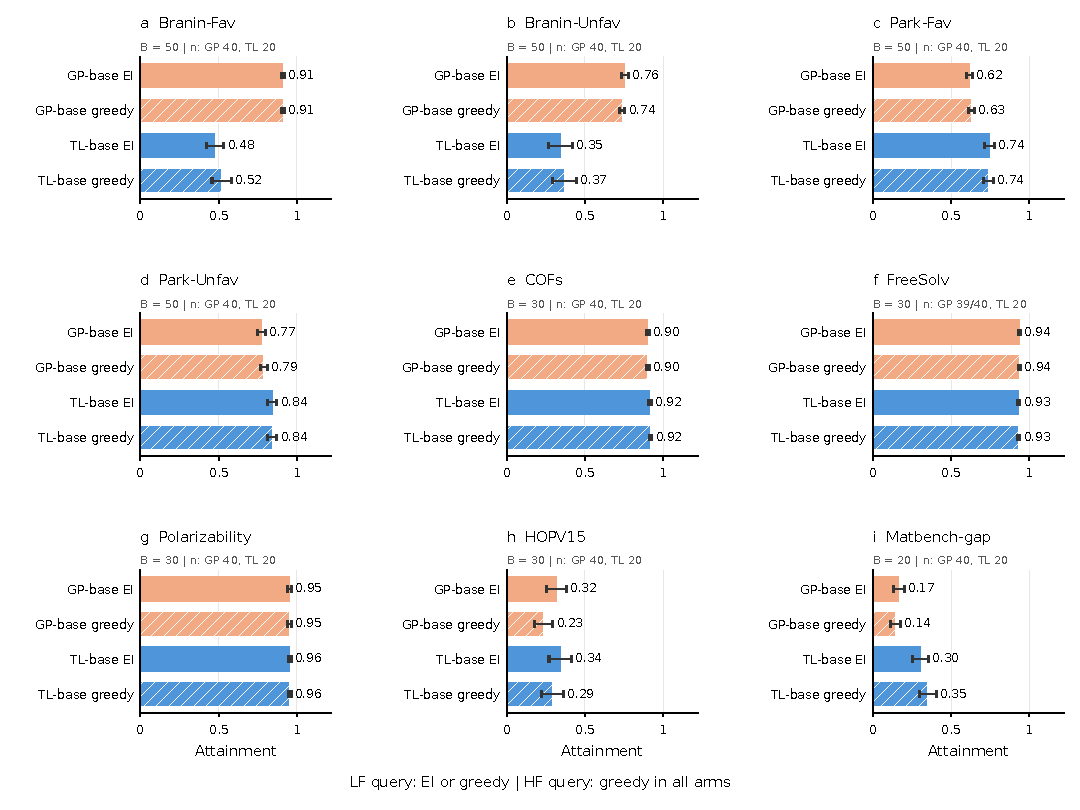
\includegraphics[width=\textwidth]{paper_figures/supp_acq_matrix.pdf}
\caption{Matched-acquisition comparison for GP-base and TL-base. \textbf{a--i,} Attainment under expected improvement (EI, solid bars) and greedy selection (hatched bars) for LF queries. HF queries use greedy selection in every arm. Orange denotes GP-base and blue denotes TL-base. Attainment follows Fig.~1, averaging the share of the budget window spent at or below the pool's top 5, 2, 1 and 0.5\% targets. Bars show mean $\pm$ s.e.\ over 40 seeds (42--81) for GP-base (39 for FreeSolv under EI) and 20 seeds (42--61) for TL-base, using the same seed set for both policies within each surrogate. Budgets match Fig.~1, except Matbench-gap at 20. TL-base values use the same runs as the EI and greedy arms in Supplementary Fig.~\ref{suppfig:portfolio}.}
\label{suppfig:acquisition}
\end{figure*}

\begin{figure*}[t]
\centering
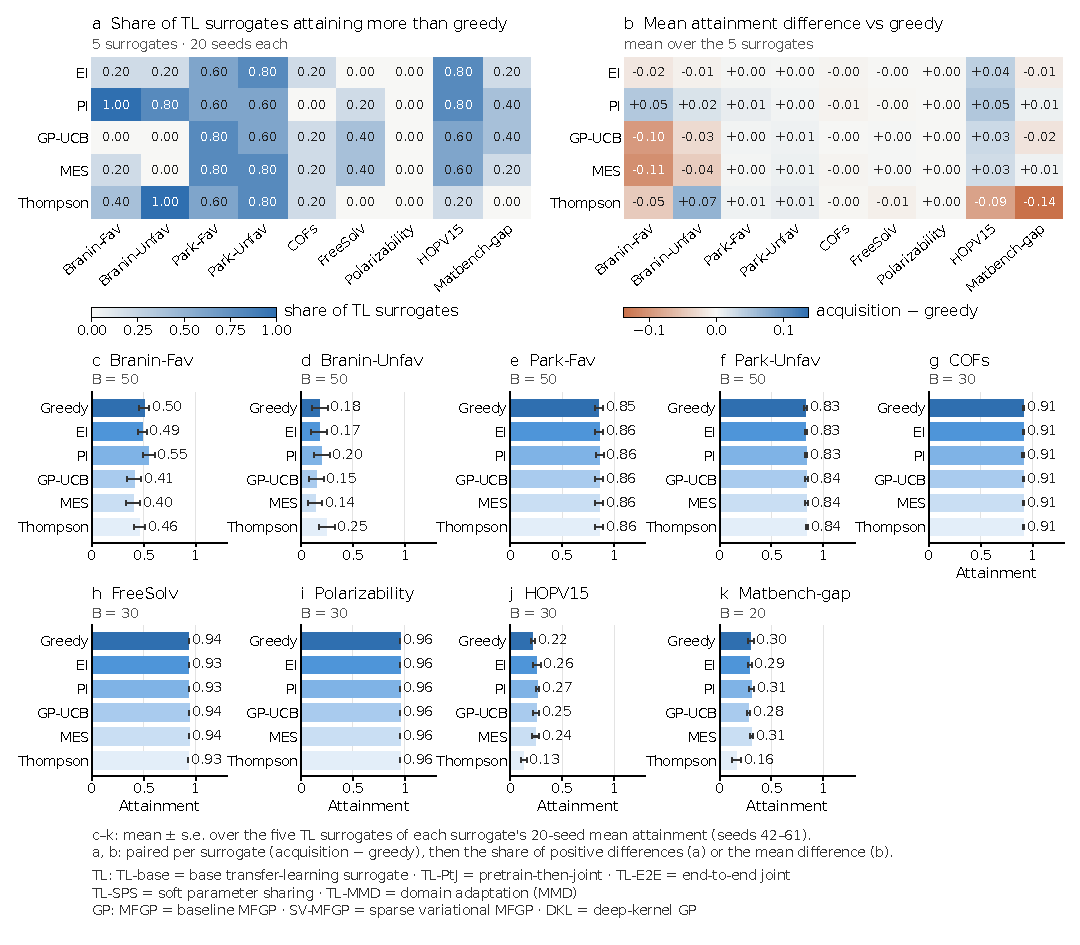
\includegraphics[width=\textwidth]{paper_figures/supp_acq_portfolio.pdf}
\caption{Acquisition portfolio under attainment. \textbf{a,} Share of the five TL surrogates whose uncertainty-driven acquisition attains more than the greedy policy on each benchmark. The acquisitions are EI, probability of improvement, the GP lower confidence bound, max-value entropy search and Thompson sampling. Each uses the BLR predictive standard deviation. \textbf{b,} Mean paired attainment difference (acquisition minus greedy) over the five surrogates. \textbf{c--k,} Attainment per acquisition, shown as mean $\pm$ s.e.\ over the five surrogates. Each surrogate value is a mean over 20 seeds (42--61). Budgets match Fig.~1, except Matbench-gap at 20.}
\label{suppfig:portfolio}
\end{figure*}


\paragraph{Calibration.} The calibration analysis of Methods~4.2 relates the loop-mean held-out LF expected calibration error (ECE) of every surrogate to its attainment from Fig.~1 (Supplementary Fig.~\ref{suppfig:calibration}a--m). Across eight surrogates and thirteen benchmarks, the correlation between loop-mean held-out LF calibration error and attainment had no consistent sign. It exceeded $|r| = 0.5$ only on Matbench-gap and ExptGap-PBE ($r = -0.67$ and $-0.90$). There, the three GPs were both the worst-calibrated LF models and the weakest optimizers. Their calibration errors spanned $0.15$--$0.36$, compared with $0.08$--$0.12$ for TL surrogates. On COFs, every surrogate attained $0.90$--$0.93$, so the small range limits interpretation of the correlation ($r = -0.48$).

Good calibration also did not identify the best optimizers. GP-base had the lowest LF calibration error on seven of thirteen benchmarks. Yet it ranked in the lower half of the eight surrogates by attainment on seven of nine molecular and materials pools. GP-DKL was the worst-calibrated on eight benchmarks but among the best optimizers on the Branin functions. ECE is averaged over refits recorded in each source run, whose horizon can differ from the attainment budget. The held-out LF calibration error uses 34--40 seeds per cell. Of 104 cells, 11 have fewer than 40. These are GP-SV on Branin-Fav and Branin-Unfav, GP-base on FreeSolv, and GP-base and GP-DKL on the four larger materials pools. For these larger pools, not every run recorded calibration error. For TL surrogates, calibration assesses the separate LF BLR head rather than the HF head driving acquisition.

\begin{figure*}[t]
\centering
%% Formerly main-text Fig. 4; moved to the SI on 2026-09-17 (letters a--m baked in).
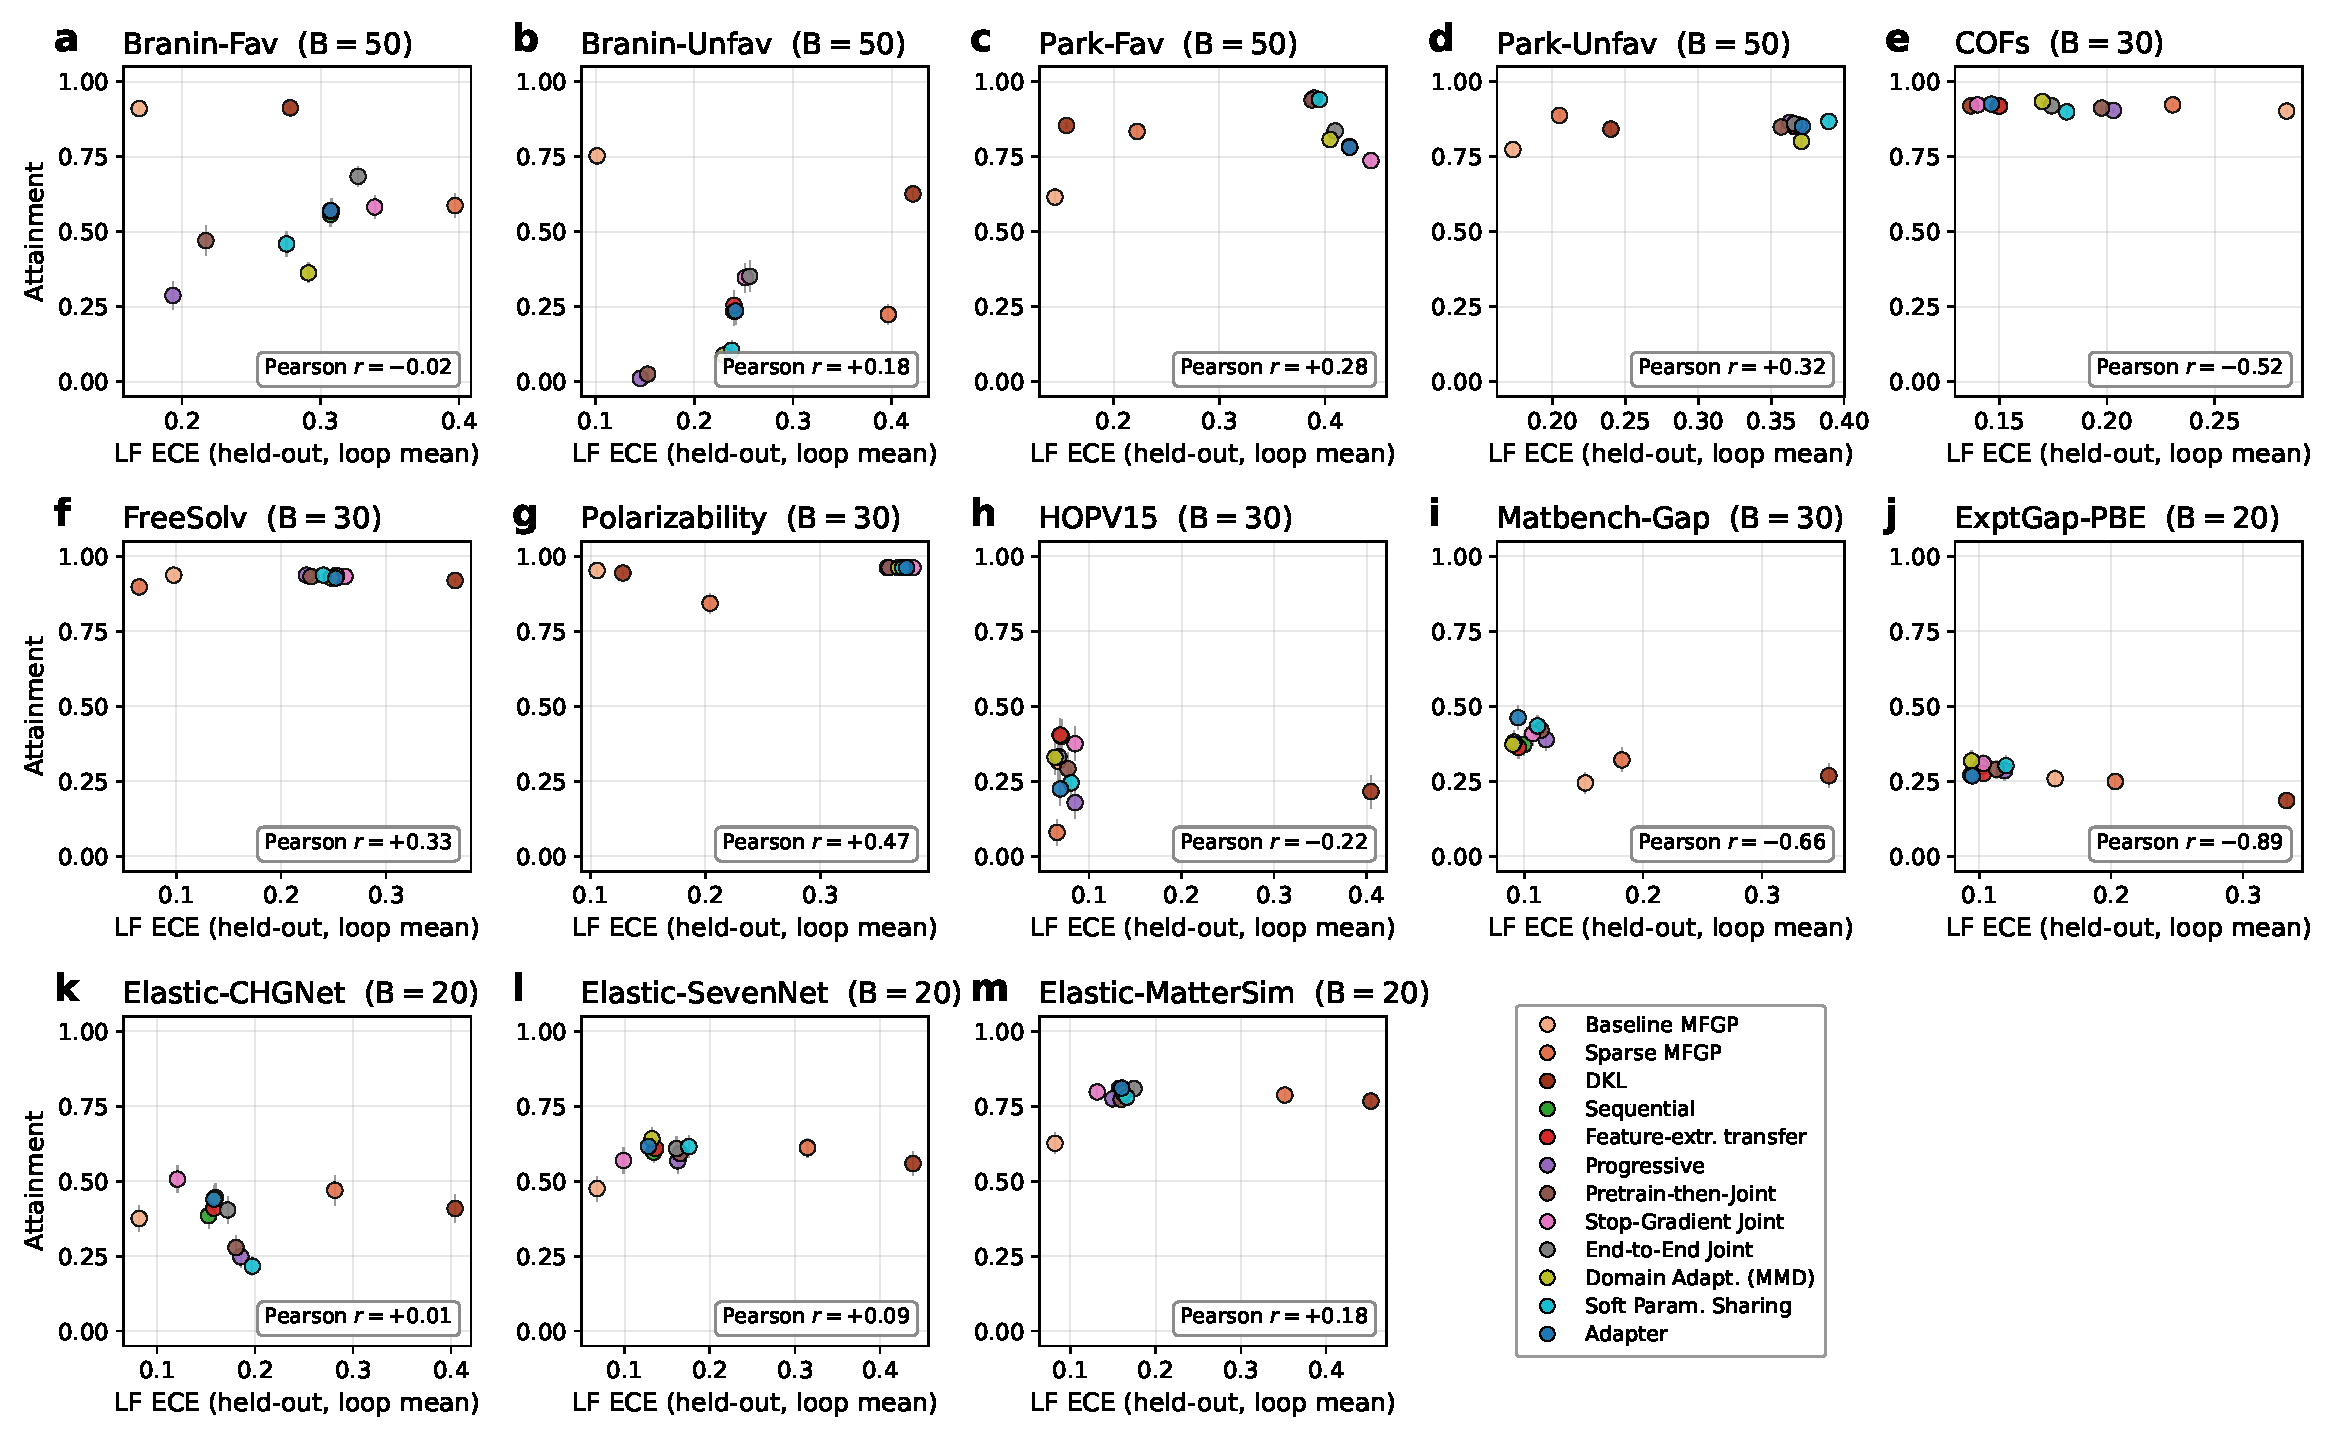
\includegraphics[width=\textwidth]{paper_figures/fig4_calibration_attain.pdf}
\caption{Calibration does not predict optimization performance.
\textbf{a--m,} Calibration versus attainment, with one panel per benchmark and one point per surrogate. Colour denotes family (orange for GPs, blue for TL), and marker denotes surrogate (legend). The horizontal axis shows held-out LF expected calibration error averaged over refits of the source runs. The vertical axis shows attainment from Fig.~1 at the displayed budget. Values are mean $\pm$ s.e.\ over 40 seeds, except 36 and 39 for GP-SV on Branin-Fav and Branin-Unfav. Each panel gives the Pearson correlation $r$ across the eight surrogate means. Because higher attainment is better, a negative $r$ associates lower calibration error with better optimization. No consistent relation appears. Only Matbench-gap and ExptGap-PBE (\textbf{i},\textbf{j}) have $|r| \ge 0.5$, and their three GP surrogates are both the worst-calibrated and least effective. On COFs, FreeSolv and Polarizability (\textbf{e}--\textbf{g}), every surrogate attains $0.84$--$0.96$. This small attainment range limits interpretation of the correlation.}
\label{suppfig:calibration}
\end{figure*}






\suppnote{Feature ablation, HF-only controls and pick logs}{suppnote:controls}

\paragraph{Feature and head-path ablations.} Supplementary Tables~\ref{supptab:feature_ablation} and~\ref{supptab:head_path} report the ablations of Methods~4.8. The head-path ablation used TL-base, whose LF prediction enters the head both as the additive offset of $\mu^{(H)}$ and as a regression column, and removed each entry point in turn with learned and with random features. Because the HF-only network has no LF network, it is listed once.

\paragraph{HF-only controls.} Supplementary Table~\ref{supptab:hf_only_baselines} compares the multi-fidelity surrogates of Fig.~1 with the two HF-only controls of Methods~4.8, a single-fidelity GP (SFGP) with EI and uniformly random HF sampling, each arm scored over its own window (definitions in the table footnotes).

\paragraph{TL-base against the GPs.} Supplementary Table~\ref{supptab:tlbase_vs_gp} lists, for every benchmark, the attainment of TL-base next to that of GP-base and of the best-performing GP on that benchmark, with the differences quoted in the main text.

\paragraph{Summary of Fig.~1o,p.} Supplementary Table~\ref{supptab:fig1_summary} lists each surrogate's mean attainment and mean deficit to the best surrogate, averaged over the thirteen benchmarks and over the nine molecular and materials benchmarks.

\paragraph{Pick logs.} Supplementary Table~\ref{supptab:hopv15_picklog} summarizes the HF pick logs of the HOPV15 runs in Fig.~2h, using the four statistics defined in Methods~4.8 and mean final regret.

\begin{table}[p]
\centering
\scriptsize
\caption{Feature ablation of the five TL surrogates on nine molecular and materials pools. Values are mean attainment over 40 seeds at $B = 30$, using the targets and window of Fig.~1. `Learned' is the reported surrogate. `Random features' replaces the head's 64-dimensional representation with features from an untrained network of the same architecture, retaining the scalar LF prediction. The `Scalar head' uses only that scalar prediction. The `HF-only network' uses the same architecture, training cost, head and initial HF points, but fits HF observations alone. It spends the whole budget on HF evaluations and contains no LF network, so it is listed once (--, not applicable).}
\label{supptab:feature_ablation}
\begin{tabular}{@{}lcccc@{}}
\toprule
Pool & Learned & Random features & Scalar head & HF-only network \\
\midrule
\multicolumn{5}{@{}l}{\emph{TL-base}} \\
COFs & 0.92 & 0.92 & 0.92 & 0.72 \\
FreeSolv & 0.93 & 0.93 & 0.93 & 0.77 \\
Polarizability & 0.96 & 0.96 & 0.96 & 0.92 \\
HOPV15 & 0.38 & 0.40 & 0.34 & 0.32 \\
Matbench-gap & 0.41 & 0.35 & 0.44 & 0.17 \\
ExptGap-PBE & 0.41 & 0.38 & 0.36 & 0.32 \\
Elastic-CHGNet & 0.62 & 0.60 & 0.50 & 0.39 \\
Elastic-SevenNet & 0.69 & 0.74 & 0.68 & 0.41 \\
Elastic-MatterSim & 0.87 & 0.88 & 0.88 & 0.39 \\
\addlinespace
\multicolumn{5}{@{}l}{\emph{TL-PtJ}} \\
COFs & 0.91 & 0.91 & 0.91 & -- \\
FreeSolv & 0.93 & 0.93 & 0.93 & -- \\
Polarizability & 0.96 & 0.96 & 0.96 & -- \\
HOPV15 & 0.29 & 0.26 & 0.22 & -- \\
Matbench-gap & 0.42 & 0.40 & 0.39 & -- \\
ExptGap-PBE & 0.38 & 0.40 & 0.35 & -- \\
Elastic-CHGNet & 0.38 & 0.35 & 0.42 & -- \\
Elastic-SevenNet & 0.70 & 0.70 & 0.67 & -- \\
Elastic-MatterSim & 0.85 & 0.86 & 0.85 & -- \\
\addlinespace
\multicolumn{5}{@{}l}{\emph{TL-E2E}} \\
COFs & 0.92 & 0.92 & 0.92 & -- \\
FreeSolv & 0.94 & 0.93 & 0.93 & -- \\
Polarizability & 0.96 & 0.96 & 0.96 & -- \\
HOPV15 & 0.33 & 0.41 & 0.38 & -- \\
Matbench-gap & 0.38 & 0.37 & 0.40 & -- \\
ExptGap-PBE & 0.36 & 0.39 & 0.41 & -- \\
Elastic-CHGNet & 0.51 & 0.52 & 0.54 & -- \\
Elastic-SevenNet & 0.73 & 0.75 & 0.71 & -- \\
Elastic-MatterSim & 0.88 & 0.88 & 0.88 & -- \\
\addlinespace
\multicolumn{5}{@{}l}{\emph{TL-SPS}} \\
COFs & 0.90 & 0.90 & 0.90 & -- \\
FreeSolv & 0.94 & 0.94 & 0.94 & -- \\
Polarizability & 0.96 & 0.96 & 0.96 & -- \\
HOPV15 & 0.25 & 0.26 & 0.16 & -- \\
Matbench-gap & 0.43 & 0.45 & 0.39 & -- \\
ExptGap-PBE & 0.41 & 0.41 & 0.47 & -- \\
Elastic-CHGNet & 0.33 & 0.34 & 0.32 & -- \\
Elastic-SevenNet & 0.73 & 0.73 & 0.67 & -- \\
Elastic-MatterSim & 0.86 & 0.85 & 0.86 & -- \\
\addlinespace
\multicolumn{5}{@{}l}{\emph{TL-MMD}} \\
COFs & 0.93 & 0.94 & 0.93 & -- \\
FreeSolv & 0.93 & 0.93 & 0.92 & -- \\
Polarizability & 0.96 & 0.96 & 0.96 & -- \\
HOPV15 & 0.33 & 0.36 & 0.39 & -- \\
Matbench-gap & 0.37 & 0.42 & 0.42 & -- \\
ExptGap-PBE & 0.40 & 0.36 & 0.41 & -- \\
Elastic-CHGNet & 0.55 & 0.51 & 0.58 & -- \\
Elastic-SevenNet & 0.75 & 0.75 & 0.75 & -- \\
Elastic-MatterSim & 0.87 & 0.87 & 0.87 & -- \\
\bottomrule
\end{tabular}
\end{table}

\begin{table}[p]
\centering
\scriptsize
\caption{Head-path ablation of TL-base on nine molecular and materials pools. Values are mean attainment over 40 seeds at $B = 30$, using the targets and window of Fig.~1. The head predicts $\mu^{(H)} = g^{(L)} + w^{\top}[\,g^{(L)}, \varphi^{(L)}, 1\,]$. `Offset' denotes the additive $g^{(L)}$ term, `input' denotes the $g^{(L)}$ regression column, and `removed' zeroes both. (1) Learned features, offset and input (the reported head). (2) Learned features, offset only. (3) Learned features, input only. (4) Learned features, $g^{(L)}$ removed from the head. (5) Random features from an untrained network of the same architecture, with $g^{(L)}$ as offset and input. (6) Random features, $g^{(L)}$ removed. Columns (1) and (5) are the Learned and Random-features configurations in Supplementary Table~\ref{supptab:feature_ablation}.}
\label{supptab:head_path}
\setlength{\tabcolsep}{3pt}%
\begin{tabular}{@{}lcccccc@{}}
\toprule
 & \multicolumn{4}{c}{Learned features} & \multicolumn{2}{c}{Random features} \\
\cmidrule(lr){2-5}\cmidrule(lr){6-7}
Pool & (1) offset + input & (2) offset only & (3) input only & (4) removed & (5) offset + input & (6) removed \\
\midrule
COFs & 0.92 & 0.92 & 0.90 & 0.69 & 0.92 & 0.63 \\
FreeSolv & 0.93 & 0.94 & 0.90 & 0.70 & 0.93 & 0.51 \\
Polarizability & 0.96 & 0.96 & 0.95 & 0.92 & 0.96 & 0.73 \\
HOPV15 & 0.38 & 0.38 & 0.17 & 0.14 & 0.40 & 0.16 \\
Matbench-gap & 0.41 & 0.39 & 0.26 & 0.05 & 0.35 & 0.06 \\
ExptGap-PBE & 0.41 & 0.35 & 0.28 & 0.16 & 0.38 & 0.14 \\
Elastic-CHGNet & 0.62 & 0.63 & 0.32 & 0.20 & 0.60 & 0.19 \\
Elastic-SevenNet & 0.69 & 0.68 & 0.59 & 0.21 & 0.74 & 0.24 \\
Elastic-MatterSim & 0.87 & 0.88 & 0.78 & 0.30 & 0.88 & 0.15 \\
\bottomrule
\end{tabular}
\end{table}

\begin{table}[p]
\centering
\scriptsize
\caption{HF-only controls and multi-fidelity surrogates on thirteen benchmarks (mean over 40 seeds). SFGP EI fits a single-fidelity GP (SFGP) to HF observations and selects queries by EI. Random HF selects HF queries uniformly. Both start from the same two initial HF points as the multi-fidelity runs and spend the whole budget on HF evaluations$^{b}$. GP-base and TL-base are the multi-fidelity surrogates in Fig.~1. Attainment uses each arm's own window, from the end of its initial design to $B$$^{a}$. Final regret is the best HF regret at $B$, in each pool's objective units (GPa for elastic-modulus pools). Footnote $c$ gives exact-optimum counts.}
\label{supptab:hf_only_baselines}
\setlength{\tabcolsep}{3.2pt}%
\begin{tabular}{@{}lc cccc cccc@{}}
\toprule
& & \multicolumn{4}{c}{Attainment} & \multicolumn{4}{c}{Final regret at $B$} \\
\cmidrule(lr){3-6}\cmidrule(lr){7-10}
& & \multicolumn{2}{c}{HF-only controls} & \multicolumn{2}{c}{Multi-fidelity} & \multicolumn{2}{c}{HF-only controls} & \multicolumn{2}{c}{Multi-fidelity} \\
\cmidrule(lr){3-4}\cmidrule(lr){5-6}\cmidrule(lr){7-8}\cmidrule(lr){9-10}
Pool & $B$ & SFGP EI & Random HF & GP-base & TL-base & SFGP EI & Random HF & GP-base & TL-base \\
\midrule
Branin-Fav & 50 & 0.84 & 0.39 & 0.91 & 0.59 & 0.00 & 0.97 & 0.02 & 0.13 \\
Branin-Unfav & 50 & 0.86 & 0.35 & 0.76 & 0.35 & 0.00 & 0.91 & 0.05 & 1.16 \\
Park-Fav & 10 & 0.21 & 0.09 & 0.09 & 0.24 & 1.02 & 1.39 & 0.02 & 0.00 \\
Park-Unfav & 10 & 0.32 & 0.22 & 0.31 & 0.44 & 0.45 & 0.88 & 0.02 & 0.00 \\
COFs & 30 & 0.49 & 0.46 & 0.90 & 0.92 & 5.48 & 4.24 & 0.00 & 0.00 \\
FreeSolv & 50 & 0.37 & 0.42 & 0.97 & 0.96 & 1.38 & 0.69 & 0.02 & 0.00 \\
Polarizability & 30 & 0.61 & 0.54 & 0.95 & 0.96 & 0.11 & 0.22 & 0.00 & 0.00 \\
HOPV15 & 30 & 0.25 & 0.36 & 0.32 & 0.38 & 2.37 & 2.03 & 2.31 & 1.27 \\
Matbench-gap & 30 & 0.21 & 0.29 & 0.25 & 0.41 & 0.49 & 0.16 & 0.12 & 0.12 \\
ExptGap-PBE & 30 & 0.43 & 0.24 & 0.33 & 0.41 & 0.22 & 0.20 & 0.11 & 0.08 \\
Elastic-CHGNet & 30 & 0.24 & 0.28 & 0.49 & 0.62 & 369 & 364 & 279 & 278 \\
Elastic-SevenNet & 30 & 0.19 & 0.18 & 0.57 & 0.69 & 229 & 229 & 155 & 129 \\
Elastic-MatterSim & 30 & 0.21 & 0.25 & 0.76 & 0.87 & 371 & 360 & 250 & 244 \\
\bottomrule
\end{tabular}
\par\smallskip
{\scriptsize
$^{a}$Windows: $B = 50$ on the Branin functions, $10$ on the Park functions and $30$ on the molecular and materials pools, except FreeSolv, evaluated at $50$. The Park and FreeSolv windows therefore differ from those of Fig.~1. The HF-only arms start their window at 2 HF-equivalent units (two farthest-point-sampled HF points), the multi-fidelity arms at the end of their LF-inclusive initial design (3 to 4.5 units). On Polarizability the five TL surrogates have identical attainment and final regret.
$^{b}$SFGP EI is a BoTorch \texttt{SingleTaskGP} (Mat\'{e}rn-5/2 ARD kernel, standardized targets, library defaults) refitted to all HF observations at every step, with the next HF query chosen by EI over the pool. Random HF follows the same protocol with the HF query drawn uniformly at random from the unevaluated candidates. Neither arm queries the LF source.
$^{c}$Seeds (of 40) whose regret reached exactly zero within the window: HOPV15, Random HF 5, SFGP EI 7, TL-base 25; Matbench-gap, SFGP EI 11, Random HF 4, GP-base 6, GP-SV 5, GP-DKL 9, TL-base 10, TL-PtJ 8, TL-E2E 9, TL-SPS 6, TL-MMD 1.
}
\end{table}

\begin{table}[p]
\centering
\scriptsize
\caption{TL-base against GP-base and the best-performing GP on thirteen benchmarks. Attainment follows Fig.~1, with mean $\pm$ s.e.\ over 40 seeds at the budgets of Fig.~1. GP-SV has 36 and 39 seeds on Branin-Fav and Branin-Unfav. The best-performing GP has the highest mean attainment on that pool. The difference $\Delta$ is TL-base minus the GP named in the preceding columns. Abbreviations are as in Fig.~1.}
\label{supptab:tlbase_vs_gp}
\setlength{\tabcolsep}{4pt}%
\begin{tabular}{@{}l ccc lcc@{}}
\toprule
& & & & \multicolumn{3}{c}{Best-performing GP} \\
\cmidrule(lr){5-7}
Pool & TL-base & GP-base & $\Delta$ & Surrogate & Attainment & $\Delta$ \\
\midrule
Branin-Fav & 0.586 $\pm$ 0.039 & 0.912 $\pm$ 0.008 & $-0.326$ & GP-DKL & 0.913 $\pm$ 0.007 & $-0.327$ \\
Branin-Unfav & 0.348 $\pm$ 0.049 & 0.756 $\pm$ 0.023 & $-0.408$ & GP-base & 0.756 $\pm$ 0.023 & $-0.408$ \\
Park-Fav & 0.737 $\pm$ 0.022 & 0.615 $\pm$ 0.018 & $+0.122$ & GP-DKL & 0.854 $\pm$ 0.010 & $-0.117$ \\
Park-Unfav & 0.855 $\pm$ 0.019 & 0.774 $\pm$ 0.024 & $+0.081$ & GP-SV & 0.888 $\pm$ 0.012 & $-0.032$ \\
COFs & 0.923 $\pm$ 0.006 & 0.902 $\pm$ 0.008 & $+0.021$ & GP-SV & 0.923 $\pm$ 0.006 & $0.000$ \\
FreeSolv & 0.934 $\pm$ 0.005 & 0.938 $\pm$ 0.005 & $-0.004$ & GP-base & 0.938 $\pm$ 0.005 & $-0.004$ \\
Polarizability & 0.963 $\pm$ 0.005 & 0.954 $\pm$ 0.011 & $+0.009$ & GP-base & 0.954 $\pm$ 0.011 & $+0.009$ \\
HOPV15 & 0.376 $\pm$ 0.056 & 0.317 $\pm$ 0.063 & $+0.058$ & GP-base & 0.317 $\pm$ 0.063 & $+0.058$ \\
Matbench-gap & 0.409 $\pm$ 0.039 & 0.245 $\pm$ 0.036 & $+0.164$ & GP-SV & 0.322 $\pm$ 0.040 & $+0.088$ \\
ExptGap-PBE & 0.406 $\pm$ 0.027 & 0.333 $\pm$ 0.031 & $+0.073$ & GP-SV & 0.337 $\pm$ 0.028 & $+0.068$ \\
Elastic-CHGNet & 0.622 $\pm$ 0.041 & 0.493 $\pm$ 0.044 & $+0.129$ & GP-DKL & 0.604 $\pm$ 0.042 & $+0.018$ \\
Elastic-SevenNet & 0.691 $\pm$ 0.037 & 0.568 $\pm$ 0.039 & $+0.123$ & GP-SV & 0.725 $\pm$ 0.030 & $-0.034$ \\
Elastic-MatterSim & 0.872 $\pm$ 0.011 & 0.757 $\pm$ 0.025 & $+0.115$ & GP-SV & 0.863 $\pm$ 0.009 & $+0.009$ \\
\bottomrule
\end{tabular}
\end{table}

\begin{table}[p]
\centering
\scriptsize
\caption{Summary of Fig.~1o,p. The table gives each surrogate's mean attainment and mean deficit to the best surrogate on each benchmark. Deficit is the benchmark's highest mean attainment minus the surrogate's mean attainment. Values are mean $\pm$ s.e.\ over benchmarks. Lower deficits are better, and 0 denotes the best attainment on every benchmark. Summaries cover all thirteen benchmarks (Fig.~1o) and the nine molecular and materials benchmarks (Fig.~1p). Surrogates are sorted by the nine-benchmark deficit. Abbreviations are as in Fig.~1.}
\label{supptab:fig1_summary}
\begin{tabular}{@{}l cc cc@{}}
\toprule
& \multicolumn{2}{c}{Thirteen benchmarks} & \multicolumn{2}{c}{Nine molecular and materials benchmarks} \\
\cmidrule(lr){2-3}\cmidrule(lr){4-5}
Surrogate & Mean attainment & Mean deficit & Mean attainment & Mean deficit \\
\midrule
TL-base & 0.671 & 0.084 $\pm$ 0.038 & 0.688 & 0.013 $\pm$ 0.007 \\
TL-MMD & 0.629 & 0.126 $\pm$ 0.060 & 0.678 & 0.023 $\pm$ 0.009 \\
TL-E2E & 0.673 & 0.081 $\pm$ 0.032 & 0.668 & 0.033 $\pm$ 0.012 \\
TL-PtJ & 0.625 & 0.130 $\pm$ 0.061 & 0.649 & 0.053 $\pm$ 0.025 \\
TL-SPS & 0.631 & 0.124 $\pm$ 0.058 & 0.647 & 0.055 $\pm$ 0.032 \\
GP-DKL & 0.686 & 0.069 $\pm$ 0.016 & 0.631 & 0.070 $\pm$ 0.021 \\
GP-SV & 0.623 & 0.131 $\pm$ 0.044 & 0.619 & 0.083 $\pm$ 0.030 \\
GP-base & 0.659 & 0.096 $\pm$ 0.027 & 0.612 & 0.089 $\pm$ 0.024 \\
\bottomrule
\end{tabular}
\end{table}


\begin{table}[p]
\centering
\scriptsize
\caption{Pick-log summary on HOPV15, using 40 seeds and $B = 30$. Mid-budget is 15 HF-equivalent units. The LF-top-ranked candidate is ranked first by the proxy and has HF regret $3.90$. `Final at LF top' gives the share of seeds ending at that candidate's regret. `Improved after 15' gives the share whose best-so-far regret improved after mid-budget. `Reached zero' counts seeds, out of 40, reaching exactly zero regret by $B = 30$. `Promoted' gives the share of second-half HF picks already evaluated at LF$^{a}$. `Final regret' gives mean final regret at $B = 30$.}
\label{supptab:hopv15_picklog}
\begin{tabular}{@{}lccccc@{}}
\toprule
Surrogate & Final at LF top & Improved after 15 & Reached zero & Promoted & Final regret \\
\midrule
GP-base & 0.45 & 0.30 & 14/40 & 1.00 & 2.31 \\
GP-SV & 0.50 & 0.38 & 3/40 & 1.00 & 3.32 \\
GP-DKL & 0.15 & 0.47 & 8/40 & 0.84 & 2.61 \\
TL-base & 0.23 & 0.62 & 25/40 & 0.99 & 1.27 \\
TL-PtJ & 0.00 & 0.62 & 20/40 & 1.00 & 1.66 \\
TL-E2E & 0.23 & 0.75 & 27/40 & 1.00 & 1.20 \\
TL-SPS & 0.00 & 0.50 & 13/40 & 1.00 & 2.44 \\
TL-MMD & 0.15 & 0.55 & 22/40 & 1.00 & 1.47 \\
\bottomrule
\end{tabular}
\par\smallskip
{\scriptsize $^{a}$Second-half picks are the HF queries issued after 15 HF-equivalent units. A pick is promoted when its candidate had already been queried at LF earlier in the same run.}
\end{table}

\suppnote{Surrogate-free LF screen and screening regimes}{suppnote:screen}

The surrogate-free screen and its screening regret are defined in Methods~4.6, which also fixes the boundary between Regime~A and Regime~B at a screening regret of $0.3$. Here we place each benchmark (Fig.~4a,b).

In Regime~A, represented by Park-Fav and Polarizability, LF--HF top-1\% overlap is approximately $1$ and screening regret is at most $0.09$. The screen therefore already identifies a near-optimal candidate. In Regime~B, high global correlation can conceal poor agreement among top-ranked candidates. COFs has a Spearman rank correlation of $0.998$ but screening regret $4.52$. Although both COFs and Polarizability have $R^2 \approx 0.96$ or higher, their screening outcomes differ. HOPV15 and Matbench-gap fall in Regime~B, with screening regrets of $3.90$ and $0.91$.

The four larger materials pools also fall in Regime~B. On ExptGap-PBE, the screen misses the optimum by $1.15$~eV. The first indexed HF optimum sits at LF rank $1{,}033$ of $3{,}508$. On the elastic-modulus pools, screening regrets are $384$~GPa for Elastic-CHGNet and $369$~GPa for Elastic-SevenNet, or $74\%$ and $97\%$ of their HF ranges. Elastic-MatterSim has screening regret $3$~GPa, or $0.6\%$ of the range, with the HF optimum at LF rank 2. These related pools therefore span nearly sufficient to uninformative screening. The best TL surrogates reached similarly low regret where screening was near-optimal and improved on it where LF rankings were less useful. On COFs, every surrogate reached zero regret within the budget (Fig.~2e).

\suppnote{Computational cost: absolute FLOPs and compute ranking}{suppnote:computational_cost}

Fig.~5 shows how surrogate compute scales with problem size. Here we report the absolute loop-integrated costs in floating-point operations (FLOPs) underlying those laws, profiled as described in Methods~4.9. GP-SV and GP-DKL required up to $22$-fold and $15$-fold the cheapest TL surrogate, respectively, and GP-base up to $5.6$-fold. GP-base was the cheapest surrogate on Park-Unfav, Polarizability and HOPV15. TL-PtJ was the cheapest TL surrogate on every benchmark. Average compute ranks across the nine benchmarks, where lower is cheaper, are $1.3$ for TL-PtJ, $2.3$ for TL-SPS and $3.3$ for TL-MMD. TL-base and GP-base both rank $4.3$, followed by TL-E2E at $5.3$, GP-DKL at $7.0$ and GP-SV at $8.0$.

\begin{figure*}[t]
\centering
%%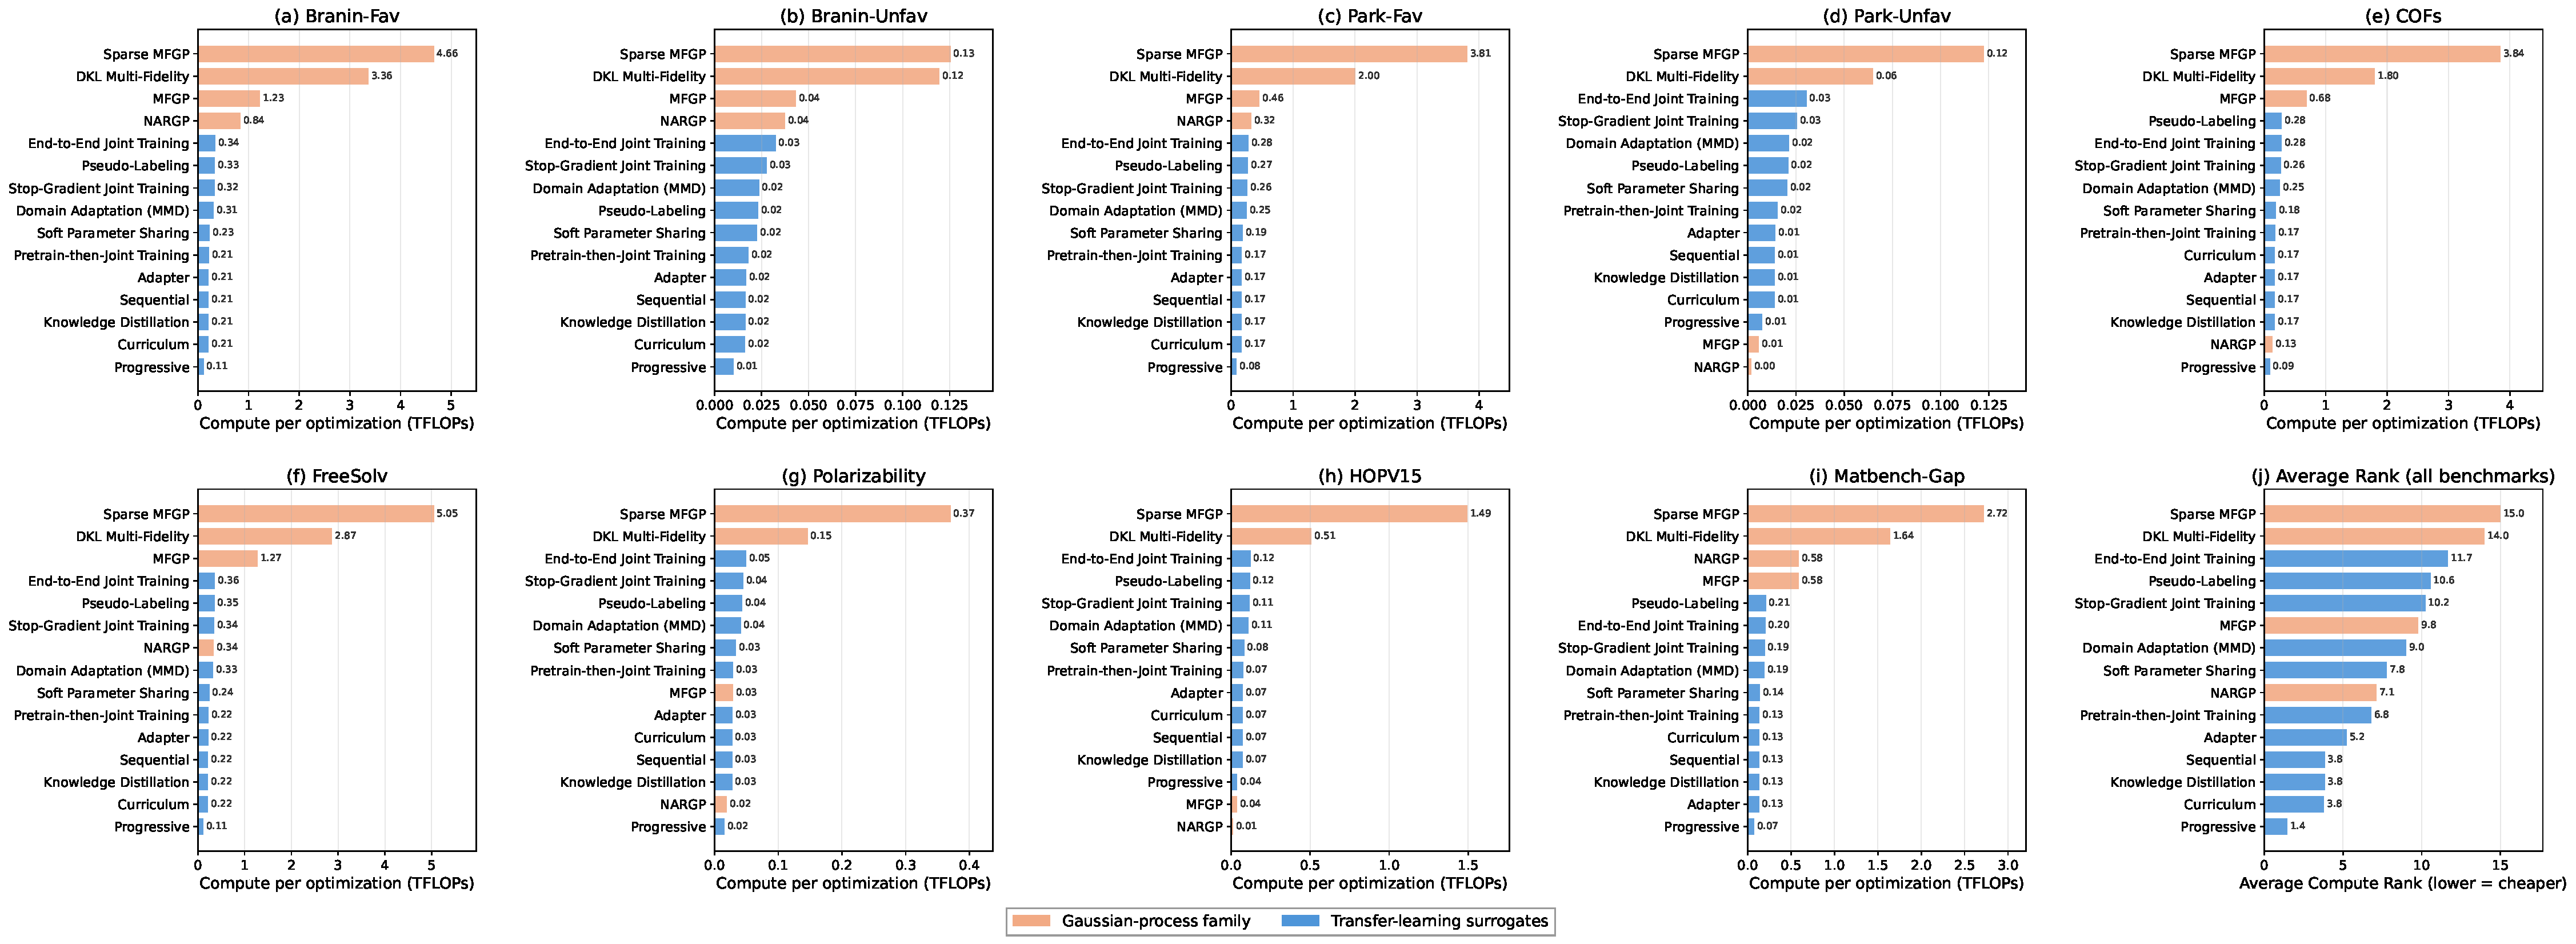
\includegraphics[width=\textwidth]{paper_figures/computing_time.pdf}
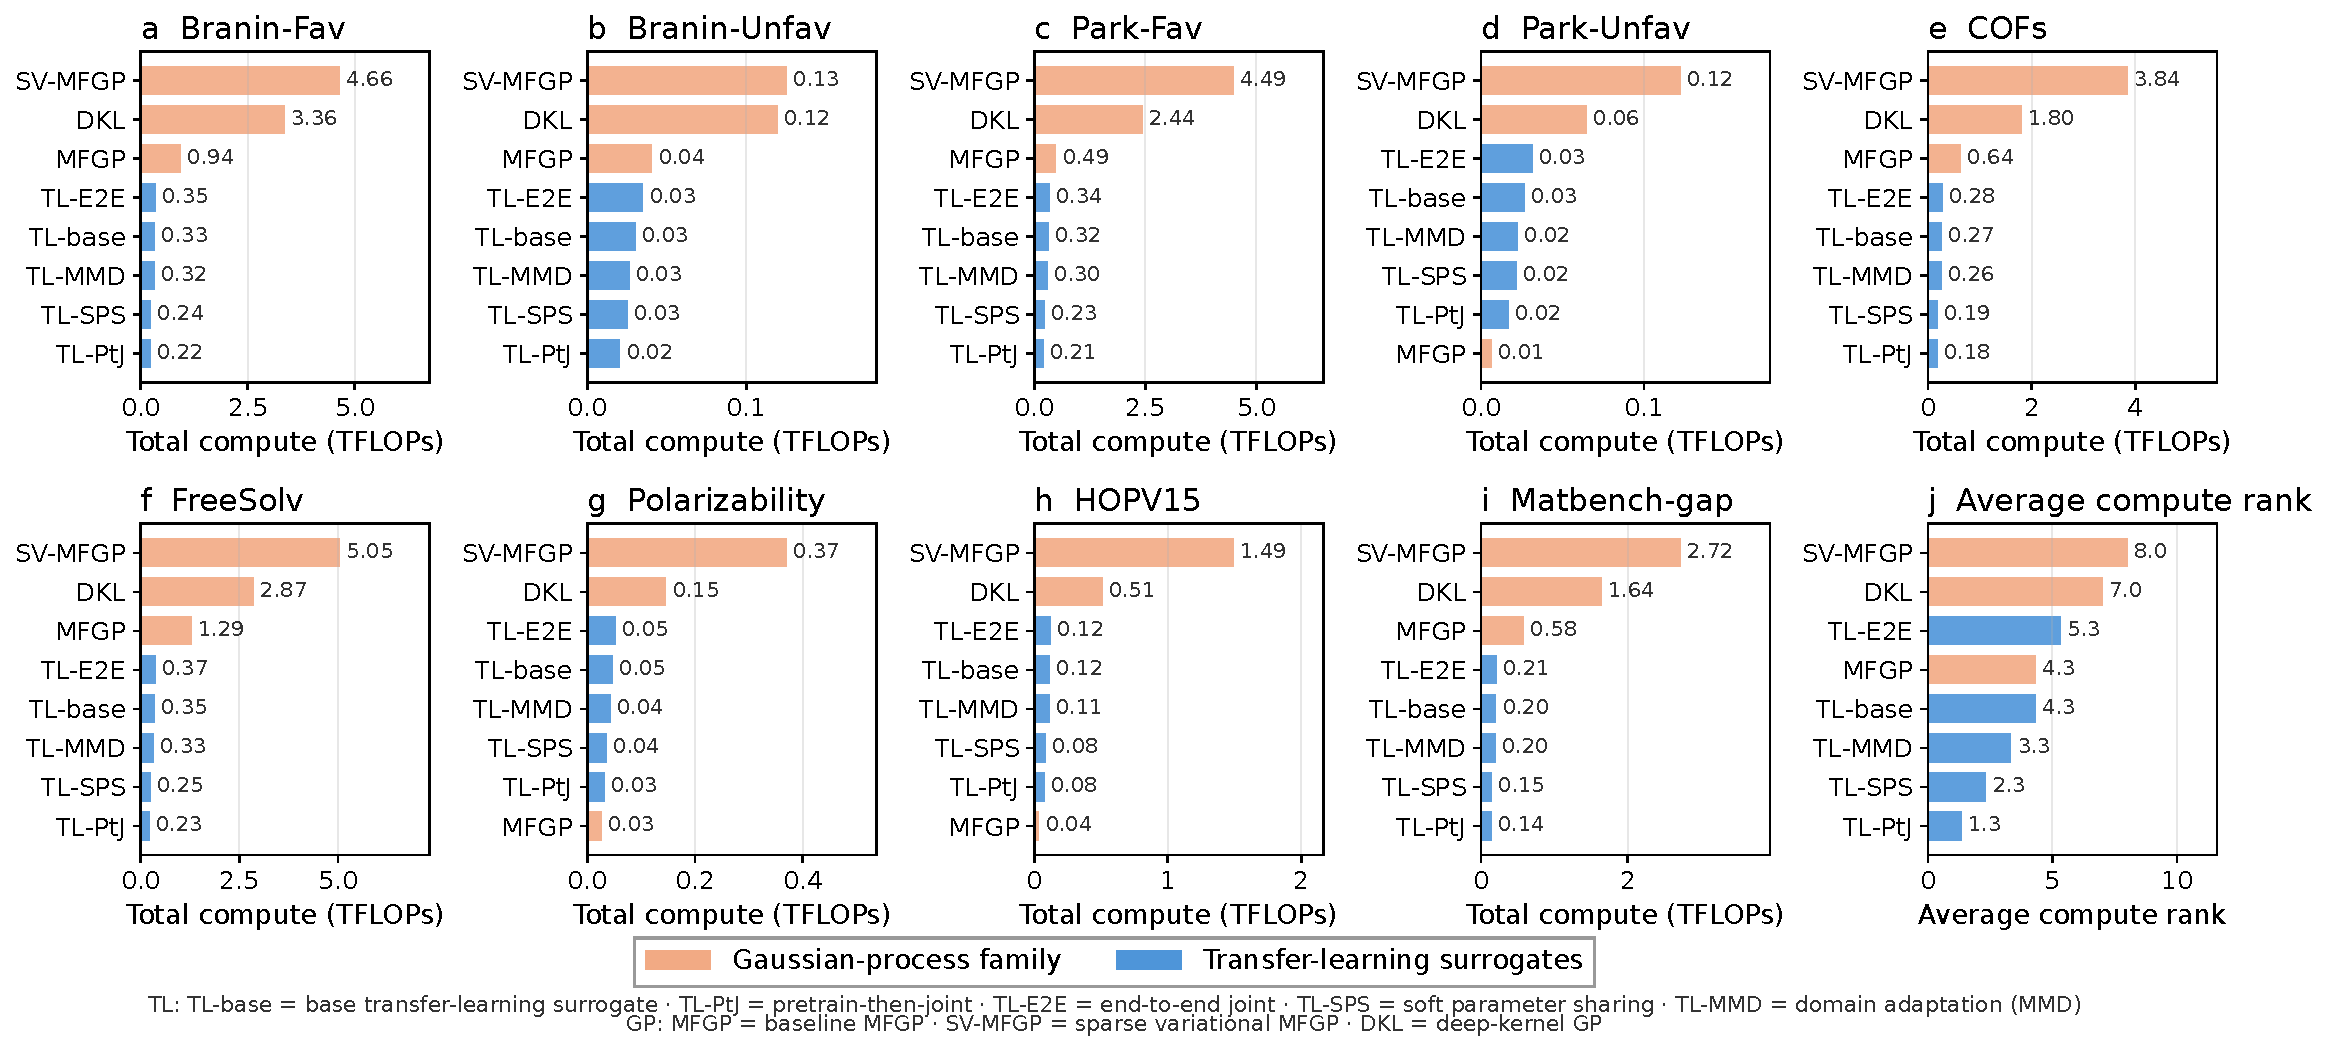
\includegraphics[width=\textwidth]{paper_figures/computing_time_blr.pdf}
\caption{Absolute computational cost across nine of the thirteen benchmarks. Hardware-independent floating-point operations (FLOPs) cover one surrogate fit and one pool-wide prediction per iteration. Costs are interpolated from profiled training-set sizes and summed over the MFBO loop. Orange denotes the GP family, and blue denotes TL surrogates. GP-SV and GP-DKL are the most expensive on every benchmark, costing up to roughly $22$-fold and $15$-fold the cheapest TL surrogate, respectively. GP-base scales as $\mathcal{O}(N^3)$ in observation count, with measured fit-FLOP exponent $k = 3.0$. TL surrogates scale as $\mathcal{O}(N)$, with $k = 0.9$--$1.0$, so the gap widens with budget. Panel \textbf{j} summarizes average compute rank across nine benchmarks, with lower values indicating lower cost. A shared legend below the panels repeats the family colours. Profiles cover all five TL surrogates and the three-member GP family, including the BLR head and residual network. Abbreviations are as in Fig.~1. FLOPs are accumulated over the budgets of Fig.~1, except FreeSolv at 50 and Matbench-gap at 20. GP-base is the cheapest surrogate on Park-Unfav, Polarizability and HOPV15.}
\label{suppfig:computing_time}
\end{figure*}




\bibliography{references}

\end{document}
